
%AIP Reprint Class%%%%%%%%%%%%%%%%%%%%%%%%%%%%%%%%%%%%%%%%%%%%%%%%%%%%%%%%%%%%%%%%%%%%%%%%%%%%%
\documentclass[aps,prl,amsmath,amssymb,reprint,superscriptaddress]{revtex4-1} %preprint version
\usepackage{graphicx}% Include figure files
\usepackage{dcolumn}% Align table columns on decimal point
\usepackage{bm}% bold math
\usepackage{epstopdf}

    \renewcommand{\topfraction}{0.9}    % max fraction of floats at top
    \renewcommand{\bottomfraction}{0.8}    % max fraction of floats at bottom
    \setcounter{topnumber}{2}
    \setcounter{bottomnumber}{2}
    \setcounter{totalnumber}{4}     % 2 may work better
    \setcounter{dbltopnumber}{2}    % for 2-column pages
    \renewcommand{\dbltopfraction}{0.9}    % fit big float above 2-col. text
    \renewcommand{\textfraction}{0.07}    % allow minimal text w. figs
    \renewcommand{\floatpagefraction}{0.7}    % require fuller float pages
    \renewcommand{\dblfloatpagefraction}{0.7}    % require fuller float pages
    \setlength{\abovecaptionskip}{5pt}
    \setlength{\belowcaptionskip}{5pt}
    \setlength{\parskip}{0pt}
    \setlength{\textfloatsep}{5pt} 

\begin{document}
\title{Observation of turbulent intermittency scaling with magnetic helicity in an MHD plasma wind-tunnel}

\author{D.A. Schaffner}
\author{A. Wan}
\author{M.R. Brown}
\affiliation{Swarthmore College, Swarthmore, PA, USA}
\date{\today}
\begin{abstract}
The intermittency in turbulent magnetic field fluctuations has been observed to scale with the amount of magnetic helicity injected into a laboratory plasma. An unstable spheromak injected into the MHD wind-tunnel of the Swarthmore Spheromak Experiment displays turbulent magnetic and plasma fluctuations as it relaxes into a Taylor state. The level of intermittency of this turbulence is determined by finding the flatness of the probability distribution function of increments for magnetic pickup coil fluctuations, $\dot{B}(t)$. The intermittency increases with the injected helicity but spectral indices are unaffected by this variation. Evidence for the role of current sheets and reconnection sites in the generation of this intermittency is provided, but the true nature of the observed intermittency remains unknown.
\end{abstract}

\maketitle

Varying levels of intermittency~\cite{frisch95} in magnetic fluctuations have been observed in many different turbulent plasmas in both space and laboratory settings. Differences in magnetic intermittent character have been seen between fast and slow solar wind turbulence~\cite{sorrisovalvo99}, at varying spatial scales in the solar wind~\cite{wan12}, at various points in the solar cycle~\cite{hnat07} and between different confinement regimes in reverse field pinches~\cite{sorrisovalvo01,marrelli05}. Simulation generated intermittency in MHD turbulence~\cite{Greco08,Greco09,Wan09,Servidio11b} compared with {\it in situ} measurements in the solar wind has suggested a link between non-Gaussian distributions of fluctuations and the presence of current sheets or reconnection layers~\cite{veltri99,carbone90}. This intermittency, or ``fat tails'' of a probability distribution function, indicates large excursions from a mean which suggests the presence of coherent structures rather than purely Gaussian fluctuations~\cite{Greco08}. Magnetic helicity, $K_{B}$, has also been an integral element of turbulence study in both observation~\cite{matthaeus82} and simulation~\cite{biskamp00,muller12}. Since the magnetic helicity of a plasma is reflective of the twistedness or knottedness of the magnetic fields, a scan of magnetic helicity can be used to vary the magnetic field structure and potentially modify the character of current sheets in the plasma. A novel experiment developed on the MHD wind-tunnel configuration of the Swarthmore Spheromak Experiment (SSX)~\cite{Gray13,schaffner14} explores this possible relationship between the observed intermittency in magnetic fluctuations and the magnetic helicity of the plasma. Given the nature of the plasma source on SSX, magnetic helicity injection can be very finely controlled and thus resulting changes in turbulent characteristics---including both spectra and intermittency---can be carefully examined.

This paper presents the results of an experimental scan which establishes a connection between a controllable experimental quantity---magnetic helicity---and a turbulent characteristic---intermittency. As the amount of injected magnetic helicity is increased, the measured flatness or kurtosis of the probability distribution function of fluctuations in a magnetic pickup coil, $dB/dt = \dot{B}(t)$, are also shown to increase ranging from near Gaussian (F$\sim 5$) to values of F $>$ 30. In contrast, the power-law behavior of the frequency spectra of these fluctuations are shown to be unaffected by this variation in helicity as shown by the power-law fit spectral indices. The scan is conducted on the wind-tunnel configuration of the Swarthmore Spheromak Experiment which consists of an 86cm long by 15.5cm wide cylindrical copper flux conserver into which a plasma gun injects dense, highly magnetized ($\sim 1\times 10^{15} cm^{-3}, \sim 5kG$) spheromak-shaped plasma that self-organizes by tilting and twisting into a Taylor state~\cite{Gray13,Matthaeus80,Taylor86}. As the plasma evolves toward a fully-relaxed Taylor state during the injection phase, the resulting turbulent magnetic field and plasma fluctuations of this transition process are measured. There is no guide or vacuum field in the chamber so the magnetic field embedded in the plasma is completely dynamical. 

The injection of magnetic helicity into the plasma is a natural consequence of the formation procedure for a plasma gun. Magnetic helicity,
%
\begin{equation}
K_{B} = \int A \cdot B dV
\label{eq:helicity_th}
\end{equation}
%
where A is magnetic potential and V is volume, is a measure of the amount of twistedness of the magnetic field lines and can be expressed in terms of square magnetic flux units (i.e. units of $Wb^{2}$). This quantity can be recast in an experimentally relevant quantity, 
%
\begin{equation}
K_{B}^{(gun)} = \int \Phi V_{gun} dt
\label{eq:helicity_exp}
\end{equation}
%
where $\Phi$ is the magnetic flux penetrating the plasma gun core and $V_{gun}$ is the voltage drop across the gun gap. An equivalence between these formulations of helicity has been shown in previous spheromak research~\cite{barnes86}; since the change in helicity is the focus of this paper, it is assumed that the value of injected helicity from equation~\ref{eq:helicity_exp} is sufficient to characterize each helicity state. It is this form of the helicity that is calculated and reported in this paper.

\begin{figure}[!htbp]
\centerline{
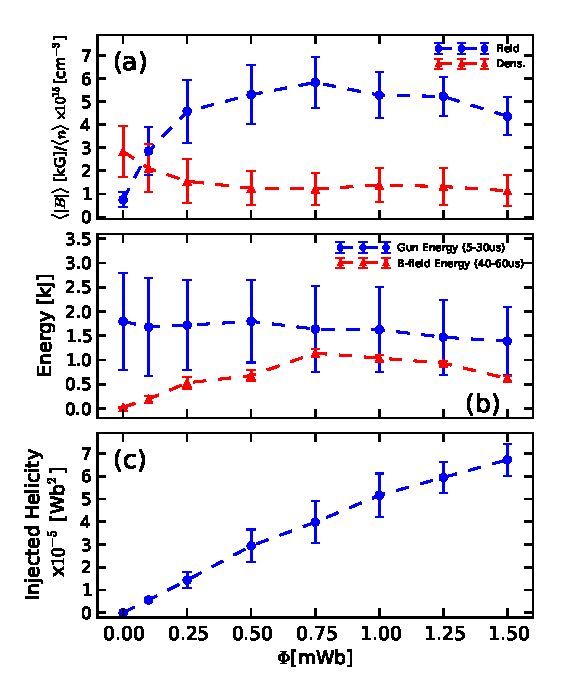
\includegraphics[width=8.5cm]{figure1.eps}}
\caption{\label{fig:helicity_scaling} (a) magnetic field magnitude (in blue) and HeNe interferometer measured line-integrated density (in red) averaged over the analysis period of 40-60$\mu s$, (b) total injected gun energy for time span of 5 to 30$\mu s$ and volume integrated magnetic field energy in the time span of 40 to 60$\mu s$, and (c) amount of helicity injected in the time span of 5 to 30$\mu s$. Error bars for all three plots indicate the standard deviation in values of magnetic field and potential (and propagated into energy and helicity) over the time range and shot number.}
\end{figure}

The injected helicity is primarily modified by the amount of magnetic flux penetrating the gun core which can be externally set between 0.0 and 1.5mWb. The gun voltage is established by a combination of the gun circuit and breakdown physics and decreases slightly as a function of changing flux, though the product of flux and voltage increases overall. The total injected helicity is computed by integrating this product from 5 to 30$\mu s$, a time frame which incorporates the helicity injection during the initial spheromak formation, and thus represents the helicity of the plasma under analysis assuming conservation of helicity. While some shots may feature multiple detachments or include field lines which do not detach from the gun---both of which can modify the equivalence of equations~\ref{eq:helicity_th} and~\ref{eq:helicity_exp}---the reported helicity values are assumed to be representative of the plasma helicity on average, and within a statistical standard deviation.

Figure~\ref{fig:helicity_scaling}(c) shows the injected helicity ensemble averaged over forty shots. The helicity scales nearly linearly with the varied magnetic flux from 0 to 7$\times 10^{-5}$Wb$^2$. Error bars indicate the standard deviation in values over time and shot number with most scatter due to fluctuations in the voltage measurement. Comparatively, figure~\ref{fig:helicity_scaling}(a) shows how the average bulk plasma features vary throughout the scan for the primary analysis period of 40-60$\mu s$: the average magnetic field at the center of the chamber grows initially with flux, but saturates around 5kG. The average density drops initially, before saturating at about 1$\times$10$^{15}$cm$^{-3}$. Figure~\ref{fig:helicity_scaling}(b) shows the energy content of the magnetic fields in relation to the amount supplied by the gun circuit. The gun energy reported is found by integrating the power, $P = I_{gun}V_{gun}$ over the same time frame as the helicity computation. The magnetic energy is calculated by finding the energy density, $B^{2}/2\mu_{0}$, at 16 radial points spanning the chamber and integrating over the volume at each location. Figure~\ref{fig:helicity_scaling} demonstrates that modifying the gun flux has little effect on the total energy content or the bulk plasma properties once a threshold helicity has been surpassed. Note that since the magnetic energy values are determined {\it during} the process of relaxation, there is no expectation of a relationship between this energy and the helicity as would be expected in a fully relaxed Taylor state.

%1mWB run
%dens 1.39e15 cm^-3
%bfield 5283 G
%Ti = 23 eV
%bulk flow = 20km/s

%results
%Va = 309km/s
%Beta = 0.07
%Cs = 31km/s
%f_i = 8MHz
%nu_i = 6MHz
%rho_i = 0.09cm
%c/w_pi = 0.61cm
%ion_mfp = 0.16cm
%doppler shifted c/wpi = 3MHz
%doppler shifted rho_i = 20MHz

\begin{table}
\caption{\label{tab:params}Typical measured and computed parameters (for $K_{B}^{(gun)}>10\mu Wb^{2}$).}
\begin{tabular}{|l|l|}
\hline
Measured&Computed\\
\hline
$\langle |B|\rangle \sim $5.2kG&$f_{ci} = $8MHz, $V_{a} = $300km/s\\
$\langle n\rangle \sim 1.4\times 10^{15}$ [cm$^{-3}$]&$c/\omega_{pi} = \delta_{i} = $0.61cm, $\rho_{i} = $0.09cm\\
$\langle T_{i}\rangle \sim $23eV&$\lambda_{mfp}^{i} = $0.16cm\\
$v_{bulk} \sim $20[km/s]&$\delta_{i}/v_{bulk} = $3Mhz \\
\hline
\end{tabular}
\end{table}

Two turbulence analysis techniques, frequency-domain power spectra and the probability distribution function (PDF) of increments~\cite{Greco09} are constructed using the magnetic pickup coil timeseries (i.e. $\dot{B}$) data. Since the probe is fabricated using a single 3mm wide loop, the $\dot{B}(t)$ signal has the best temporal resolution and bit-depth (65MHz sampling and 14-bit dynamic range) and is used directly in the analysis rather than converting the timeseries to $B(t)$ by integration. For spectra analysis, the transformed $\dot{B}(f)$ data can be scaled into $B(f)$ in frequency space by dividing the power in each frequency bin by $f^{2}$. The PDF and flatness analysis, on the other hand, uses $\dot{B}(t)$ directly. The results reflect a time span of $40$ to $60 \mu s$ after initial breakdown when the plasma is in a quasi-stationary state between formation and decay. Furthermore, an ensemble average of forty shots is recorded for each helicity state.

The wavelet power spectrum of magnetic field fluctuations for each helicity case is presented in Figure~\ref{fig:Btot_spectra}. The curves shown are constructed by taking a sixth-order Morlet wavelet transform~\cite{torrence98} of each component timeseries ($\dot{B}_r$,$\dot{B}_{\theta}$,and $\dot{B}_{z}$), squaring to get power and dividing the power in each frequency bin by $f^{2}$. The resulting component power spectra are then summed to yield total magnetic fluctuation spectra. The absolute scale in Figure~\ref{fig:Btot_spectra}(a) has been artificially staggered to clearly illustrate the shape of each curve. Each spectrum exhibits a break-point at approximately 1MHz which is hypothesized to be due to dissipation effects near the ion inertial scale, $\delta_{i} = c/\omega_{pi}$ (see Table~\ref{tab:params}). Using a Maximum Likelihood Estimation method~\cite{deWit13,clauset09}, two power-law fits are computed for linear regions (in log-log scaling) just above and below the break-point. The spectral index and error for each fit is indicated in Figure~\ref{fig:Btot_spectra}(b). Though the helicity is increasing linearly, the power-law fit for each spectrum does not change significantly, hovering around a slope of 3 for low frequency fits and around 5 for high frequency fits. This trend indicates that the change in helicity does not appear to have an effect on the frequency spectra in these regions.

\begin{figure}[!htbp]
\centerline{
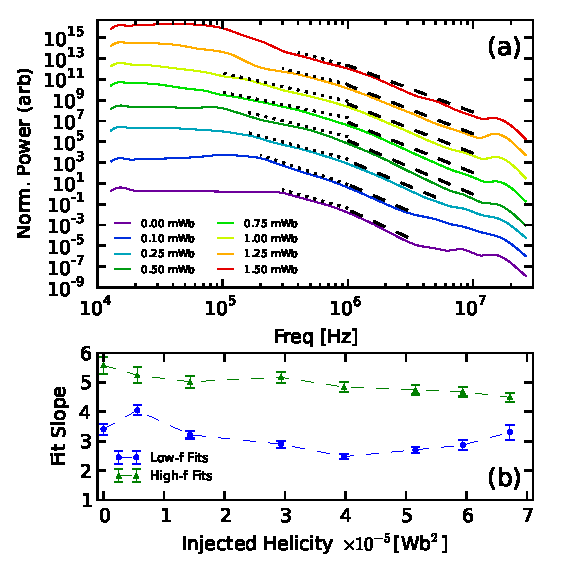
\includegraphics[width=8.5cm]{figure2.eps}}
\caption{\label{fig:Btot_spectra} (a) Total magnetic field fluctuation spectra (sum of $B_r$,$B_{\theta}$,and $B_{z}$), for each of the eight helicity states. The spectra are staggered in order to highlight the shape of each spectrum. Lines above each curve reflect the slope of the power-law fit and the range of the fit. Dotted (dashed) lines are for the fits of the low (high) frequency range. (b) Spectral indices with error of the fits for each curve for either low or high frequencies.}
\end{figure}

The calculation of spectra can be viewed as a second-order moment of the PDF of increments; since the analysis of spectra shows little change for different values of helicity, it is natural to search for potential changes at higher order moments. We now show that the nature of the intermittency in the $\dot{B}(t)$ fluctuations does appear to change with the helicity state. The PDF of increments is constructed by taking differences of values in a time signal---in this case, $\dot{B}_{r}$---separated by a time scale $\Delta t$ with the increment defined as,
\begin{equation}
\Delta \dot{B}_r \equiv \dot{B}_r(t + \Delta t)- \dot{B}_r(t).
\label{eq:increment}
\end{equation}

Figure~\ref{fig:Br_flatness} demonstrates how intermittency is determined through the measure of flatness.  Fig.~\ref{fig:Br_flatness}(a) shows the PDF of increments of a timeseries at 3$\times 10^{-5}$ Wb$^{2}$ of injected helicity for two different timescales: $0.15\mu s$ and $15\mu s$.  The PDF with small time scale shows a highly pointed distribution with broad, fat tails indicating large excursions from the mean value---or intermittency. This non-Gaussian behavior is highlighted when the PDFs are compared to a Gaussian curve. Dashed lines in Figure~\ref{fig:Br_flatness}(a) indicate the best-fit Gaussian to each distribution. The PDF with a large time scale increment clearly show a much more Gaussian distribution compared to its best fit. Similarly-shaped distributions for respective long and short timescales are observed in the solar wind~\cite{sorrisovalvo99}. The level of intermittency for each scale can be quantified by computing the normalized fourth-order moment of the PDF---also called flatness or kurtosis. The flatness for each PDF as a function of time scale and for each helicity state is shown in Fig.~\ref{fig:Br_flatness}(b). Clearly, each state shows increasing flatness, and thus intermittency, with decreasing time scale. The flatness of a purely Gaussian distribution is indicated at F=3. Moreover, it is observed that the overall flatness of each curve increases as a function of helicity. In other words, the intermittency of the plasma increases with injected helicity---this is the main result of this paper.

\begin{figure}[!htbp]
\centerline{
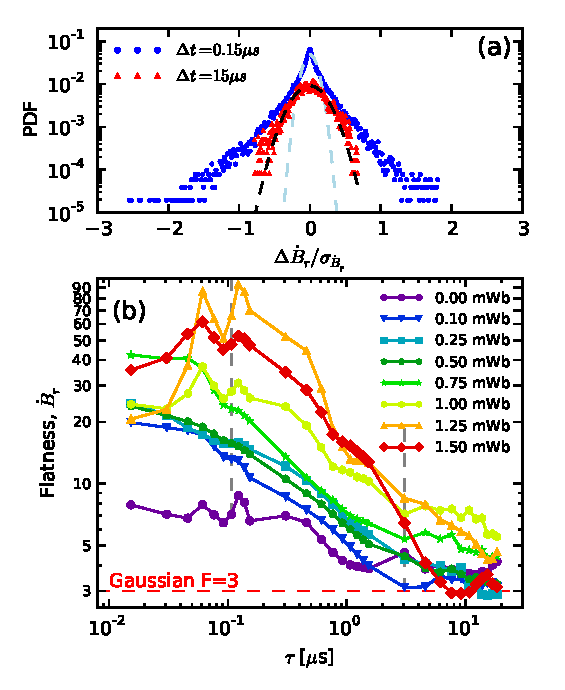
\includegraphics[width=8.5cm]{figure3.eps}}
\caption{\label{fig:Br_flatness} (a) PDFs for a long and short $\Delta t$ from data for $K_{B}^{(gun)} = 3\times 10^{-5}$ Wb$^{2}$ indicating the change in intermittency with timescale. Dashed lines indicate the best-fit Gaussian curves for each PDF. (b) Flatness values for each timescale and each helicity state for the radial $\dot{B}$ component.}
\end{figure}

This change with helicity is summarized in Figure~\ref{fig:flatness_scaling}(a) where the calculated flatness of $\dot{B}_{r}$, as shown in the curves of Fig.~\ref{fig:Br_flatness}(b) as well as those for $\dot{B}_{\theta}$ and $\dot{B}_{z}$ has been averaged between the scales indicated by the dashed gray lines: between $0.1\mu s$ and $3.0\mu s$, which approximately corresponds to a frequency range of 333kHz to 10MHz. This region is where the frequency spectra are generally linear in the logarithmic scaling of Figure~\ref{fig:Btot_spectra}(a). The average flatness increases with helicity, although there is a brief trend reversal at about 1.5$\times 10^{-5}$ Wb$^{2}$ before the curve begins to increase again.

\begin{figure}[!htbp]
\centerline{
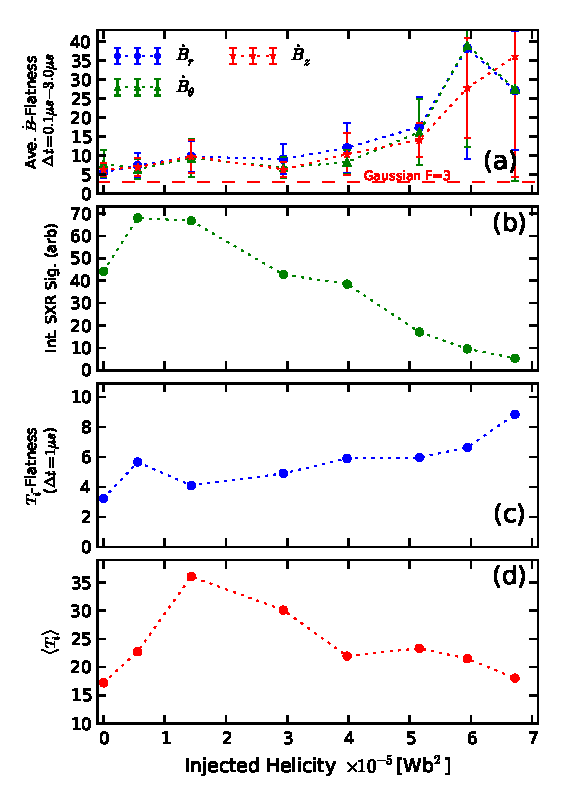
\includegraphics[width=8.5cm]{figure4.eps}}
\caption{\label{fig:flatness_scaling} (a) Flatness of magnetic component increments averaged over timescales from 0.1$\mu s$ to 3.0$\mu s$ vs helicity. Error bars reflect the standard deviation of the computed average and primarily indicate that the spread in flatness values from large to small time differences tends to grow with helicity. (b) Integrated soft X-ray signal versus helicity. (c) Flatness of $T_{i}$ time series versus helicity. (d) Average $T_{i}$ versus helicity.}
\end{figure}

While the physical origin of this observed intermittency and its trend with helicity is not completely understood in the context of this experiment, investigation of intermittency in space plasma yields some possible explanations. Simulations of MHD plasmas modeled after solar wind plasma with time series extracted in ways to match that of \textit{in-situ} satellite observation~\cite{Greco08,Greco09}, have indicated a correlation between intermittency and the passing of current sheets or reconnection sites. Past experiments on SSX have focused on observation of reconnection layers~\cite{Gray10,brown12}; thus, the experiment has a number of diagnostics designed to measure signatures of reconnection including a set of soft X-ray photo-diodes~\cite{chaplin09} to measure X-rays generated by fast electrons and an ion Doppler spectrometer (IDS) system that measures bursts of ion temperature, $T_{i}$, and ion flow~\cite{brown12}. Figure.~\ref{fig:flatness_scaling}(b-d) shows the output of these diagnostics for the same helicity scan and limited to the same time range as the turbulence data presented above. Soft X-ray measurement shows an initial increase in x-ray light going from zero to small amounts of helicity, but then a consistent decrease in measured light. Fig.~\ref{fig:flatness_scaling}(c) shows the flatness of PDFs constructed from $T_{i}(t)$ as a function of helicity. Like, the flatness curve of $\dot{B}$, the $T_{i}$ intermittency also increases with helicity. Meanwhile, the average, or background, $T_{i}$ does not vary much, peaking slightly between 1 and 2$\times 10^{-5}$ Wb$^{2}$, but generally maintaining a value of between 20-25eV. 

Taken together, these trends can be viewed as evidence for a connection between intermittency and reconnection. The hypothesis is that increasing the injected helicity increases the number of reconnection sites during Taylor relaxation (more $T_{i}$ bursts) but decreases their size (less X-ray light from electron acceleration). Given past observations of some of these effects in more controlled reconnection experiments on SSX~\cite{brown12}, it is reasonable to think similar mechanisms are at play here as well. Alternate explanations, however, can involve helicity-related modification of fluctuations at the ion scale as a mechanism for the observed heating~\cite{wu13,osman11}. Unfortunately, these hypotheses cannot be fully tested without higher spatial resolution (current spectroscopy diagnostics are line-integrated) and better temporal resolution in the ion measurements. In addition to improving diagnostics, comparisons to simulation may help as is done in solar wind research.

This paper presents the observation of a clear change in the intermittent character of $\dot{B}$ fluctuations as a function of injected helicity while simultaneously showing little to no change in the turbulent frequency-domain power spectra. Though the spectra presented here are not direct evidence of the turbulent energy cascade process, the results suggest that the cascade process is not modified by the level of helicity in the plasma. The discrepancy between spectra and PDF results is also an indication of the need to study higher order moments in turbulence analysis (i.e. 4th order Flatness vs 2nd order spectra) in order to fully flesh out modifications in turbulence~\cite{matthaeusVelli11}. The experiment demonstrates a straightforward method for modifying the intermittency in a plasma for detailed study and highlights an advantage of turbulence research in an experimental setting as a complement to {\it in-situ} space measurements and simulation. A possible connection to a physical mechanism was established through soft X-ray and IDS measurements, which suggested the intermittency is related to the spatial size of reconnection sites in the plasma. However, given the limitations of the current diagnostics, definitive conclusions cannot be made, but do provide impetus for further comparison to simulation in this experimental configuration~\cite{schaffner14} as well as more exploration as to the effects of helicity on the turbulence~\cite{biskamp00}.

Finally, since helicity observations have been made in many of the same turbulent plasmas that exhibit intermittency~\cite{goldstein94, ji95, telloni12}, a link between helicity and turbulent intermittency may be a useful metric for understanding turbulence in both space and experiment, including possible comparisons to the variation of intermittency as a function of solar distance~\cite{greco12} as well as differences between confinement regimes in fusion devices.

The authors gratefully acknowledge many useful discussions with and comments from W.H. Matthaeus and V.S. Lukin. This work is supported by DOE OFES and NSF CMSO.

\providecommand{\noopsort}[1]{}\providecommand{\singleletter}[1]{#1}%
\begin{thebibliography}{99}

\bibitem{frisch95}Frisch, U. 1995, {\it Turbulence} (Cambridge: Cambridge Univ. Press)

\bibitem{sorrisovalvo99}Sorriso-Valvo, L. {\it et al.} Geophys. Res. Lett. {\bf 26}, 1801–1804 (1999).

\bibitem{wan12}Wan, M. {\it et al.} ApJ. {\bf 744} 177 (2012).

\bibitem{hnat07}Hnat, B. {\it et al.} Geophys. Res. Lett. {\bf 34} L15108 (2007).

\bibitem{sorrisovalvo01}Sorriso-Valvo, L. {\it et al.} Planet. Space Sci. {\bf 49}, 1193–1200 (2001).

\bibitem{marrelli05}Marrelli, L. {\it et al.} Phys. Plasmas. {\bf 12}, 030701 (2005).

\bibitem{Greco08}Greco, A. {\it et al.} Geophys. Res. Lett. {\bf 35}, L19111 (2008).

\bibitem{Greco09}Greco, A. {\it et al.}, ApJ {\bf 691}, L111 (2009).

\bibitem{Wan09}Wan, M. {\it et al.} Phys. Plasmas {\bf 16}, 080703 (2009).

\bibitem{Servidio11b}Servidio, S. {\it et al}, J. Geophys. Res. {\bf 116}, A09102 (2011).

\bibitem{veltri99}P. Veltri. Plasma Phys. Cont. Fusion. {\bf 41} A787 (1999).

\bibitem{carbone90}V. Carbone, P. Veltri and A. Mangeney. Phys. Fluids A. {\bf 2} 1487 (1990).

\bibitem{matthaeus82}Matthaeus, W.H. and Goldstein, M.L. J. Geophys. Res. {\bf 87} 6011 (1982).

\bibitem{biskamp00}Biskamp, D. and M$\ddot{\mathrm{u}}$ller, W-C. Phys. Plas. {\bf 7} 4889 (2000).

\bibitem{muller12}M$\ddot{\mathrm{u}}$ller, W-C., Malapaka, S.K., and Busse, A. Phys. Rev. E. {\bf 85} 015302(R) (2012).

\bibitem{Gray13}T. Gray, M. R. Brown, and D. Dandurand. Phys. Rev. Lett. {\bf 110}, 085002 (2013). 

\bibitem{schaffner14}D.A. Schaffner {\it et al.} Plasma Phys. Cont. Fus. {\bf 56} 064003 (2014).

\bibitem{Taylor86}Taylor, J.B. Rev. Mod. Phys. {\bf 58}, 741 (1986).

\bibitem{Matthaeus80}Matthaeus,W.H. and Montgomery,D. Ann. N.Y. Acad. Sci. {\bf 357}, 203 (1980).

\bibitem{barnes86}C.W. Barnes {\it et al.} Phys. Fluids {\bf 29} 3415 (1986).

\bibitem{torrence98}Torrence, C. and Compo, G.P. Bull. Am. Meteorol. Soc. {\bf 79}, 6178 (1998).

\bibitem{deWit13}Dudok de Wit, T., {\it et al.} Space Sci. Rev. {\bf 0038-6308}, p. 1-29 (2013).

\bibitem{clauset09}Clauset, A., Rohilla Shalizi, C. and Newman, M.E.J. SIAM Rev. {\bf 51}, 661703 (2009).

\bibitem{Gray10}Gray,T. {\it et al.} Phys. Plasmas {\bf 17}, 102106 (2010).

\bibitem{chaplin09}Chaplin, V.H., {\it et al.} Phys. Plasmas {\bf 16} 042505 (2009).

\bibitem{brown12}Brown, M.R. {\it et al.} Phys. Plasmas {\bf 19} 080704 (2012).

\bibitem{wu13}P. Wu {\it et al.} Phys. Rev. Lett. {\bf 111} 121105 (2013).

\bibitem{osman11}K.T. Osman {\it et al.}. ApJ Lett. {\bf 727} L11 (2011).

\bibitem{matthaeusVelli11}Matthaeus, W.H. and Velli, M. Space Sci. Rev. {\bf 160} 145-168 (2011).

\bibitem{goldstein94}Goldstein, M.L., Roberts, D.A. and Fitch, C.A. Jour. Geo. Res. {\bf 99} 11519-11538 (1994).

\bibitem{ji95}Ji, H., Prager, S.C. and Sarff, J.S. Phys. Rev. Lett. {\bf 74} 2945 (1995).

\bibitem{telloni12}Telloini, D. {\it et al.}. ApJ. {\bf 751} 19 (2012).

\bibitem{greco12}A. Greco {\it et al.} ApJ. {\bf 749} 105 (2012).

\end{thebibliography}

\end{document}

